\chapter{Ergebnisse und Auswertung}
\label{ch:results}

Alle 1920 Benchmark-Läufe der in \cref{ss:test-matrix} definierten Testmatrix wurden erfolgreich abgeschlossen; kein einzelner Lauf musste verworfen werden. Sämtliche im Folgenden genannten Messwerte sind, sofern nicht durch eine eigene Abbildung oder Tabelle im Fließtext belegt, in \cref{tab:appendix-benchmark} im Anhang vollständig dokumentiert. Ab $n = 8000$ ist die Messstreuung (IQR) in mehreren Szenarien sichtbar erhöht. Als wahrscheinlichste Ursache kommen die Browser-internen Störeinflüsse (\cref{sss:gc-interference,sss:jit-interference}) in Betracht, die sich nicht vollständig kontrollieren lassen.

\section{H2: Scripting-Aufwand pro Tick bei steigender UI-Dichte}
\label{s:results-h2}

\subsection{Scripting-Zeit, Overhead-Faktor und Frequenzeinfluss}
\label{ss:results-h2-scripting}

Mit zunehmender UI-Dichte~$n$ steigen die medianen \textit{scriptingMsPerTick}-Werte beider Frameworks stetig an (\cref{fig:h2-scripting}a). Die Kurve von React verläuft dabei durchgehend steiler als die von Svelte; bei $n = 10\,000$ und $f = 10\,\text{Hz}$ beträgt die Scripting-Zeit für React $11{,}2\,\text{ms}$ gegenüber $4{,}1\,\text{ms}$ für Svelte. Ab $n \geq 8000$ erhöht sich die Messstreuung (IQR) deutlich, was auf die in \cref{sss:gc-interference,sss:jit-interference} diskutierten browserinternen Störeinflüsse zurückgeführt werden kann. Der in \cref{fig:h2-scripting}b gezeigte Overhead-Faktor (Verhältnis von React- zu Svelte-Scripting-Zeit) wächst bei $f = 10\,\text{Hz}$ mit zunehmendem~$n$: Der relative Scripting-Mehraufwand von React gegenüber Svelte nimmt mit steigender UI-Dichte zu. Beide Frameworks weisen zwar eine Skalierung von $O(n)$ auf (\cref{ss:expected-scaling,sss:runes-overhead}), unterscheiden sich jedoch im Aufwand pro Element. Reacts Reconciliation verarbeitet bei jeder Zustandsänderung stets den gesamten betroffenen Teilbaum, unabhängig davon, wie viele Knoten tatsächlich verändert wurden (\cref{ss:expected-scaling}). Zusätzlich werden bei jedem Render-Vorgang erneut React-Elemente erzeugt. Sveltes feingranulare Reaktivität begrenzt den Aufwand hingegen auf die tatsächlich betroffenen Abhängigkeiten (\cref{sss:finegraned-reactivity}), was den Aufwand pro Element reduziert (\cref{sss:runes-overhead}). Für $f = 10\,\text{Hz}$ weisen beide Frameworks bei jeder $n$-Stufe nahezu identische Rendering-Zeiten auf: Bei $n = 4000$ erreichen beide $4{,}74\,\text{ms}$ pro Tick; bei $n = 10\,000$ betragen die Werte $13{,}31\,\text{ms}$ (React) gegenüber $13{,}55\,\text{ms}$ (Svelte, Abweichung $1{,}8\,\%$). Der messbare Unterschied zwischen den Frameworks liegt bei dieser Frequenz somit überwiegend im Scripting (\cref{ss:profiling-categories}). Die INP-Phasenzerlegung (\cref{ss:results-h1-phases}) zeigt bei $f = 10\,\text{Hz}$ allerdings einen deutlichen Unterschied in der \textit{presentationDelay} ($51{,}9\,\text{ms}$ vs.\ $78{,}1\,\text{ms}$). Dieser Unterschied wird durch die Rendering-Zeit pro Tick nicht erfasst; die Ursache lässt sich mit den erhobenen Metriken nicht eindeutig bestimmen (vgl.~\cref{s:limitations}). Bei $f = 20\,\text{Hz}$ treten jedoch Unterschiede auf: Für $n = 10\,000$ betragen die Rendering-Zeiten $11{,}87\,\text{ms}$ (React) beziehungsweise $13{,}71\,\text{ms}$ (Svelte), was einer Abweichung von $15\,\%$ entspricht. Als mögliche Ursache kommt Sveltes Effect-Batching in Betracht (\cref{sss:microtasks}): Die gebündelten DOM-Updates werden innerhalb eines einzigen Microtasks abgearbeitet, ohne dass verbleibende Arbeit auf spätere Frames verteilt wird (\cref{sss:scheduling-priotising-of-updates}). Dadurch könnte der Rendering-Aufwand bei $f = 20\,\text{Hz}$ pro Tick gebündelt anfallen. React hingegen gibt durch kooperatives Yielding (\cref{sss:scheduling-priotising-of-updates}) die Kontrolle zwischen einzelnen Fiber-Schritten an den Browser zurück. Der genaue Mechanismus lässt sich anhand der vorliegenden Daten nicht eindeutig bestimmen. Der Rendering-Unterschied ist bei $f = 20\,\text{Hz}$ am größten ($15\,\%$) und gleicht sich bei $f \approx 62\,\text{Hz}$ nahezu aus ($4{,}95\,\text{ms}$ vs.\ $4{,}92\,\text{ms}$). Mit steigender Tick-Frequenz nimmt die Scripting-Zeit pro Tick insgesamt ab, jedoch nicht gleichförmig und nicht gleich stark bei beiden Frameworks. Bei Svelte steigt die Scripting-Zeit bei $n = 10\,000$ von $4{,}12\,\text{ms}$ ($10\,\text{Hz}$) zunächst auf $4{,}29\,\text{ms}$ ($20\,\text{Hz}$) an, bevor sie auf $3{,}66\,\text{ms}$ ($62\,\text{Hz}$) fällt. Für React ($n = 10\,000$) fällt \textit{scriptingMsPerTick} von $11{,}2\,\text{ms}$ ($10\,\text{Hz}$) auf $3{,}42\,\text{ms}$ ($62\,\text{Hz}$): ein Rückgang um $70\,\%$. Für Svelte sinkt der Wert im selben Bereich von $4{,}1\,\text{ms}$ auf $3{,}66\,\text{ms}$ (Rückgang um $11\,\%$). Beide Frameworks nähern sich mit steigender Frequenz einem gemeinsamen Mindestaufwand an: dem durch die $O(n)$-Komplexität bedingten Basisaufwand, den keine Laufzeitoptimierung unterschreiten kann ($\lceil n \cdot 0{,}05 \rceil$ Signal-Auswertungen bzw.\ die Fiber-Reconciliation, vgl.\ \cref{sss:runes-overhead}). Da Reacts Ausgangswert bei niedrigen Frequenzen weiter von diesem Minimum entfernt liegt als der von Svelte, fällt der relative Rückgang für React entsprechend größer aus. Der große React-Rückgang deutet auf frequenzabhängig wegfallenden Overhead hin, möglicherweise durch JIT-Optimierungen auf häufig ausgeführten Code-Pfaden (\cref{sss:jit-interference}). Sveltes geringer Rückgang ergibt sich daraus, dass der Spielraum nach unten von vornherein klein ist. Der genaue Mechanismus lässt sich ohne V8-internes Profiling nicht bestimmen. Bei $f \approx 62\,\text{Hz}$ und $n = 10\,000$ ergibt sich dadurch ein Scripting-Schnittpunkt: React erreicht $3{,}42\,\text{ms}$ (IQR $0{,}13\,\text{ms}$), Svelte $3{,}66\,\text{ms}$ (IQR $0{,}10\,\text{ms}$); damit ist Svelte hier erstmals geringfügig langsamer als React. Auffällig ist, dass Reacts Scripting-Zeit bei $f \approx 62\,\text{Hz}$ von $n = 8000$ ($3{,}53\,\text{ms}$) auf $n = 10\,000$ ($3{,}42\,\text{ms}$) leicht zurückgeht, während sie bei allen anderen Frequenzen durchgehend mit~$n$ wächst. Da der Unterschied von $0{,}11\,\text{ms}$ kleiner ist als der IQR beider Messpunkte ($n = 8000$: $0{,}20\,\text{ms}$; $n = 10\,000$: $0{,}13\,\text{ms}$), lässt er sich nicht sicher vom Messrauschen unterscheiden. Der Scripting-Schnittpunkt ergibt sich daher überwiegend aus Sveltes $O(n)$-Angleichung (\cref{sss:runes-overhead}) und dem ungleichmäßigen frequenzabhängigen Rückgang im Scripting, nicht dadurch, dass Reacts Scripting-Zeit gestiegen wäre. Damit schränkt der Scripting-Schnittpunkt H2 ein, ohne H2 zu widersprechen. Die Rendering-Zeiten verlaufen bei $n = 10\,000$ uneinheitlich. Bereits bei $f = 10\,\text{Hz}$ sind sie nahezu identisch. Nach dem Maximum des Abstands bei $f = 20\,\text{Hz}$ fallen die React-Werte stetig: von $13{,}31\,\text{ms}$ ($10\,\text{Hz}$) über $11{,}87\,\text{ms}$ ($20\,\text{Hz}$) und $8{,}40\,\text{ms}$ ($30\,\text{Hz}$) auf $4{,}95\,\text{ms}$ ($62\,\text{Hz}$). Sveltes Werte bleiben zunächst bei $13{,}55\,\text{ms}$ ($10\,\text{Hz}$) bzw. $13{,}71\,\text{ms}$ ($20\,\text{Hz}$), bevor sie über $9{,}45\,\text{ms}$ ($30\,\text{Hz}$) auf $4{,}92\,\text{ms}$ ($62\,\text{Hz}$) abfallen. Bei $f \approx 62\,\text{Hz}$ nähern sich beide Frameworks einem gemeinsamen Wert von ca. $4{,}9\,\text{ms}$ an. Der genaue Mechanismus dieser frequenzabhängigen Abnahme lässt sich anhand der vorliegenden Messdaten nicht eindeutig bestimmen.
\begin{figure}[H]
  \centering
  \begin{minipage}[t]{\textwidth}
    \centering
    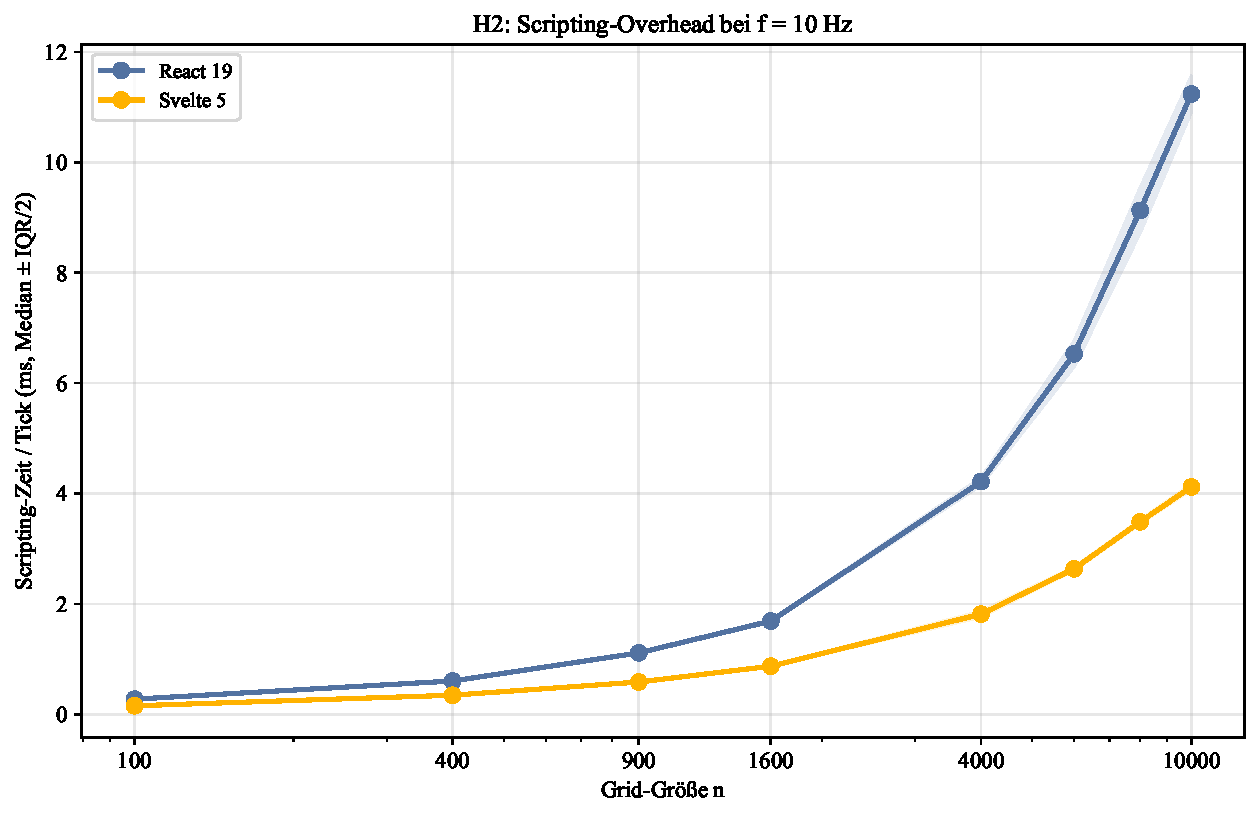
\includegraphics[width=\textwidth,keepaspectratio]{bilder/h2_scripting}
    \subcaption{Scripting-Zeit (Median\,±\,IQR) bei $f = 10\,\text{Hz}$}
    \label{fig:h2-scripting-abs}
  \end{minipage}
  \vspace{1.5em}
  \begin{minipage}[t]{\textwidth}
    \centering
    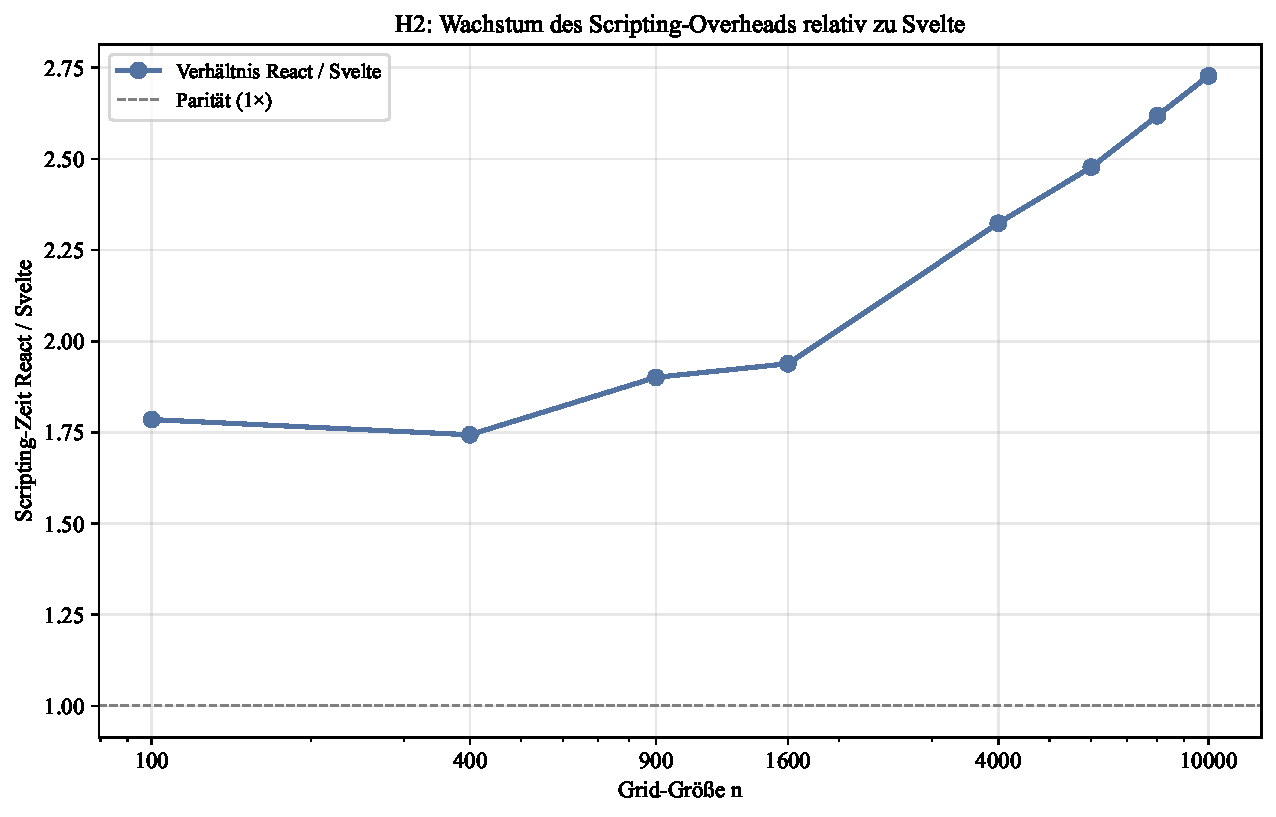
\includegraphics[width=\textwidth,keepaspectratio]{bilder/h2_scripting_ratio}
    \subcaption{Overhead-Faktor React\,/\,Svelte über $n$ bei $f = 10\,\text{Hz}$}
    \label{fig:h2-scripting-ratio}
  \end{minipage}
  \caption[H2 – Scripting-Auswertung beider Frameworks bei $f = 10\,\text{Hz}$]{H2 – Scripting-Auswertung: (a) mediane \textit{scriptingMsPerTick} beider
           Frameworks bei $f = 10\,\text{Hz}$; (b) Quotient React\,/\,Svelte bei
           $f = 10\,\text{Hz}$ über alle $n$-Stufen (vgl.~\cref{ss:profiling-categories}).}
  \label{fig:h2-scripting}
\end{figure}

\subsection{Bewertung von H2}
\label{ss:results-h2-verdict}

Bei $f \leq 30\,\text{Hz}$ bestätigen die Messdaten H2: Der Scripting-Aufwand pro Tick von React wächst mit steigendem~$n$ stärker als der von Svelte, was auf die Reconciliation-Kosten der Fiber-Architektur und die feingranulare Reaktivität von Svelte zurückzuführen ist (\cref{sss:fiber-engine-structure,sss:runes-overhead}). Anzumerken ist, dass sich der genaue Anteil der Compiler-Memoisierung an diesen Scripting-Kosten im gewählten Versuchsaufbau nicht isolieren lässt (vgl.~\cref{s:limitations}). Hinzu kommt, dass bei $f \approx 30\,\text{Hz}$ der Abstand im letzten $n$-Intervall ($n = 8000$ auf $n = 10\,000$) von $3{,}94\,\text{ms}$ auf $3{,}35\,\text{ms}$ zurückgeht: Sveltes Scripting-Zuwachs ($+0{,}79\,\text{ms}$) übersteigt dort den von React ($+0{,}20\,\text{ms}$). Da der Unterschied von $0{,}59\,\text{ms}$ jedoch innerhalb der Summe der IQR-Werte beider Frameworks bei $n = 8000$ liegt (React-IQR: $0{,}40\,\text{ms}$, Svelte-IQR: $0{,}19\,\text{ms}$), lässt er sich nicht sicher vom Messrauschen unterscheiden. Bei $f \approx 62\,\text{Hz}$ gilt H2 nur eingeschränkt: Svelte erreicht bei $n = 10\,000$ mit $3{,}66\,\text{ms}$ erstmals eine höhere Scripting-Zeit als React ($3{,}42\,\text{ms}$). Dieser Scripting-Schnittpunkt lässt sich durch zwei Faktoren erklären: die in \cref{sss:runes-overhead} beschriebene $O(n)$-Angleichung, die bei steigendem $n$ auch bei einer Mutationsrate von $5\,\%$ je Tick praktisch wirksam wird, sowie den ungleichmäßigen frequenzabhängigen Scripting-Rückgang (\cref{ss:results-h2-scripting}). \textbf{H2 wird teilweise bestätigt.}

\section{H3: Speichereffizienz unter Dauerlast}
\label{s:results-h3}

\subsection{Qualitative Heap-Analyse: Dominator-Struktur im Dev-Build}
\label{ss:results-h3-qualitative}

Heap-Snapshots bei $n = 100$ im Development-Build zeigen die internen Datenstrukturen beider Frameworks in lesbarer Form (\cref{sss:qualitative-heap}). \Cref{fig:heap-structures} stellt die aufgeklappten Objekte gegenüber; \cref{tab:heap-qualitative} fasst die abgelesenen Größen zusammen.
\begin{table}[htbp]
  \centering
  \caption[Qualitative Heap-Analyse: interne Objekt-Strukturen ($n = 100$, Dev-Build)]{Qualitative Heap-Analyse: interne Objekt-Strukturen bei $n = 100$
           im Development-Build (Chrome DevTools, Heap-Snapshot nach
           Benchmark-Abschluss)}
  \label{tab:heap-qualitative}
  \small
  \begin{tabular}{lrr}
    \toprule
    \textbf{Metrik}
      & \textbf{React 19} (\texttt{FiberNode})
      & \textbf{Svelte 5} (Signal-POJO) \\
    \midrule
    Instanzen ($n = 100$)  &  423      &  103      \\
    Shallow Size gesamt    & 60{,}9\,kB &  5{,}8\,kB \\
    Retained Size gesamt   & 131\,kB   & 19{,}8\,kB \\
    \bottomrule
  \end{tabular}
  \par\smallskip
  \raggedright\footnotesize
  \textit{Anmerkung:} Shallow Size pro Objekt (berechnet als Gesamt\,÷\,Anzahl):
  React $\approx 144$\,B, Svelte\,5 $\approx 56$\,B.
  Quelle: Chrome DevTools Memory-Tab, Summary-Ansicht, Dev-Build
  (\texttt{localhost:5173} bzw.\ \texttt{localhost:5174}, \texttt{gridSize=100}).
\end{table}
\begin{figure}[H]
  \centering
  \begin{subfigure}{\textwidth}
    \centering
    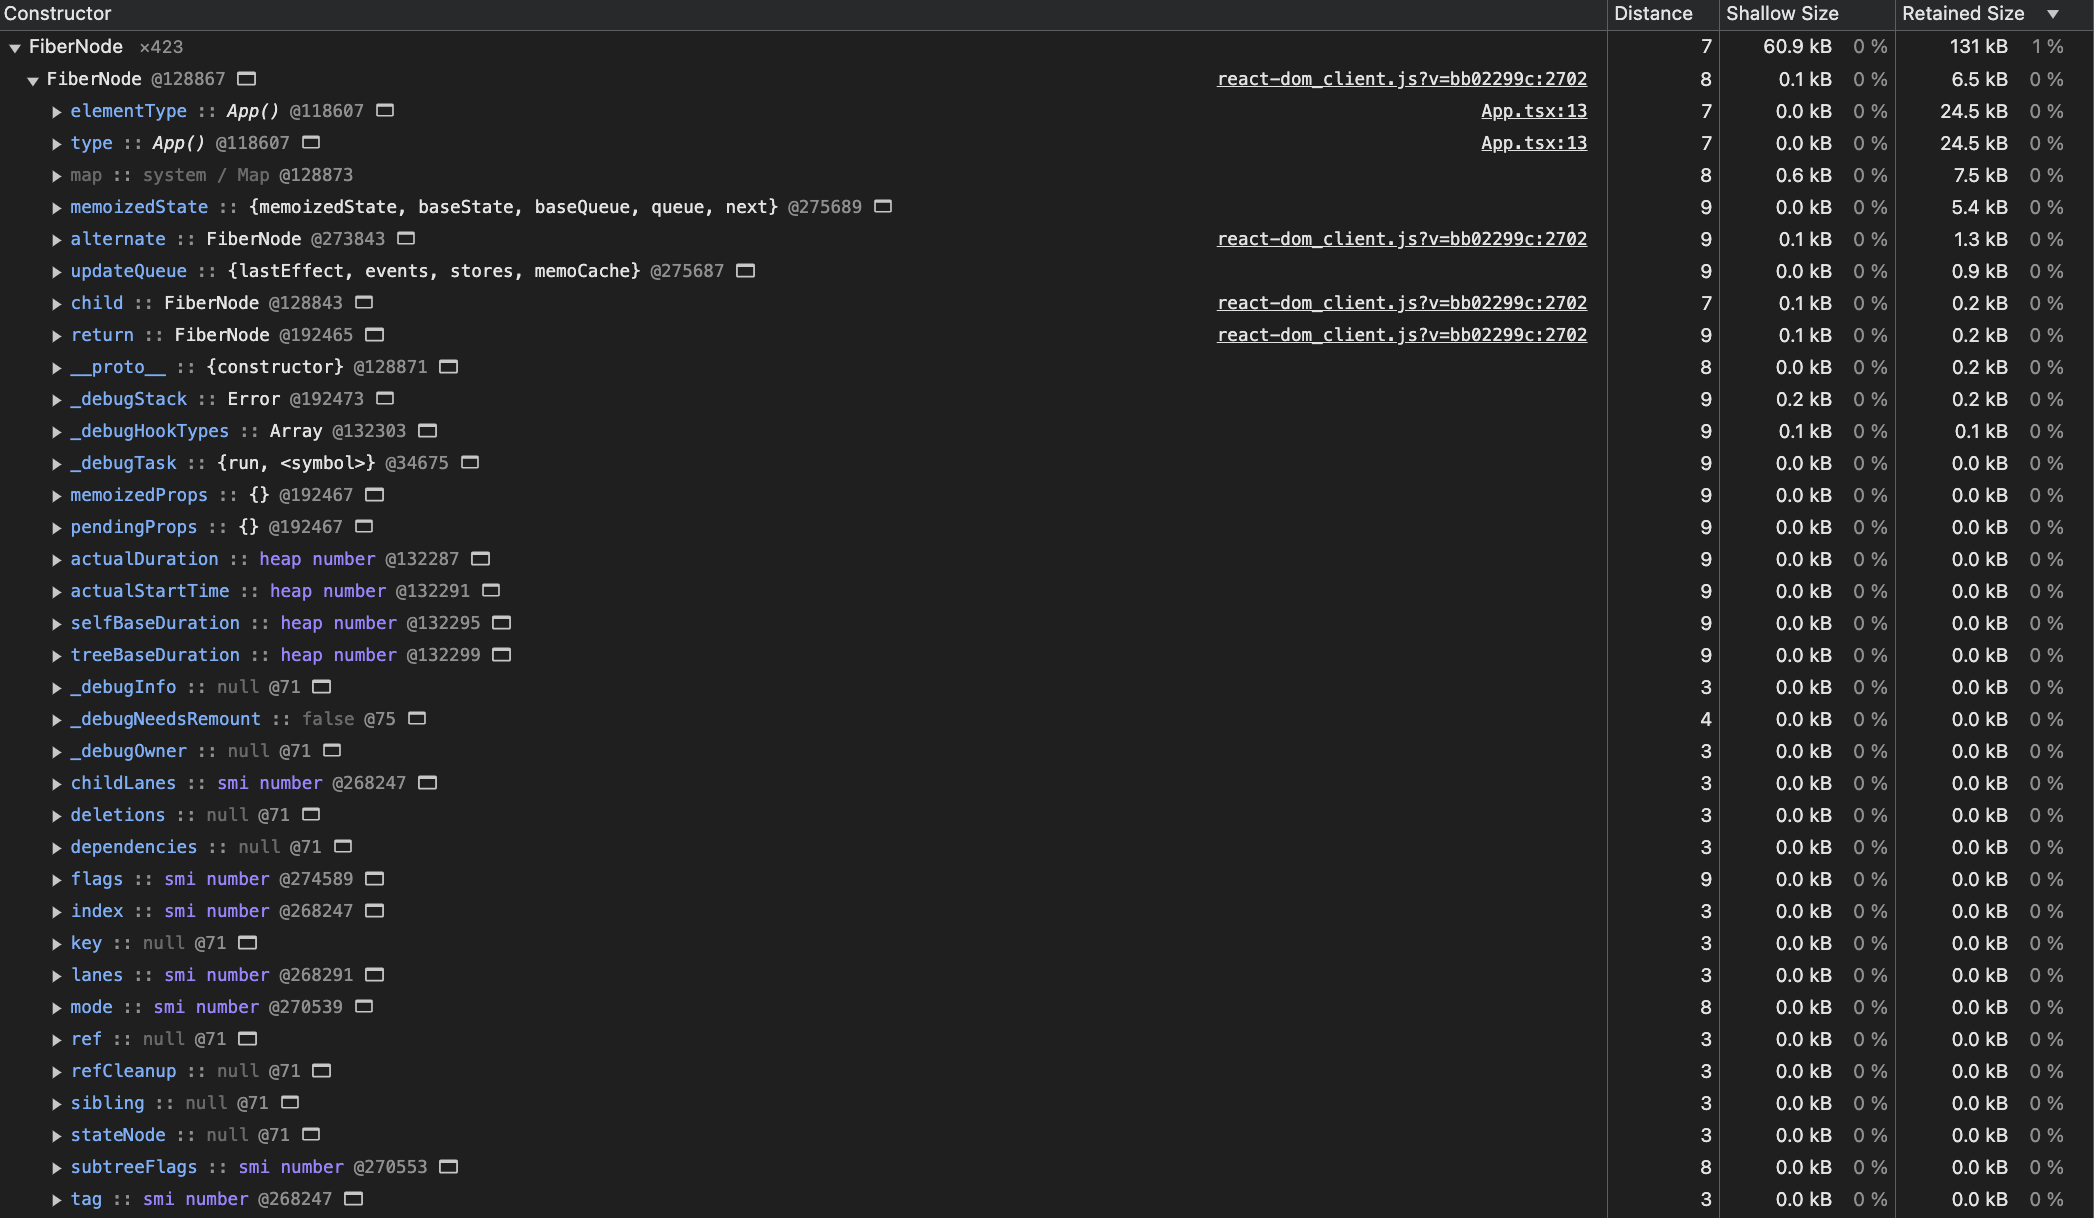
\includegraphics[width=\textwidth]{bilder/heap-react-fibertree}
    \subcaption{React 19: \texttt{FiberNode}-Instanz mit allen Feldern}
    \label{fig:heap-react}
  \end{subfigure}
  \vspace{0.5em}
  \begin{subfigure}{\textwidth}
    \centering
    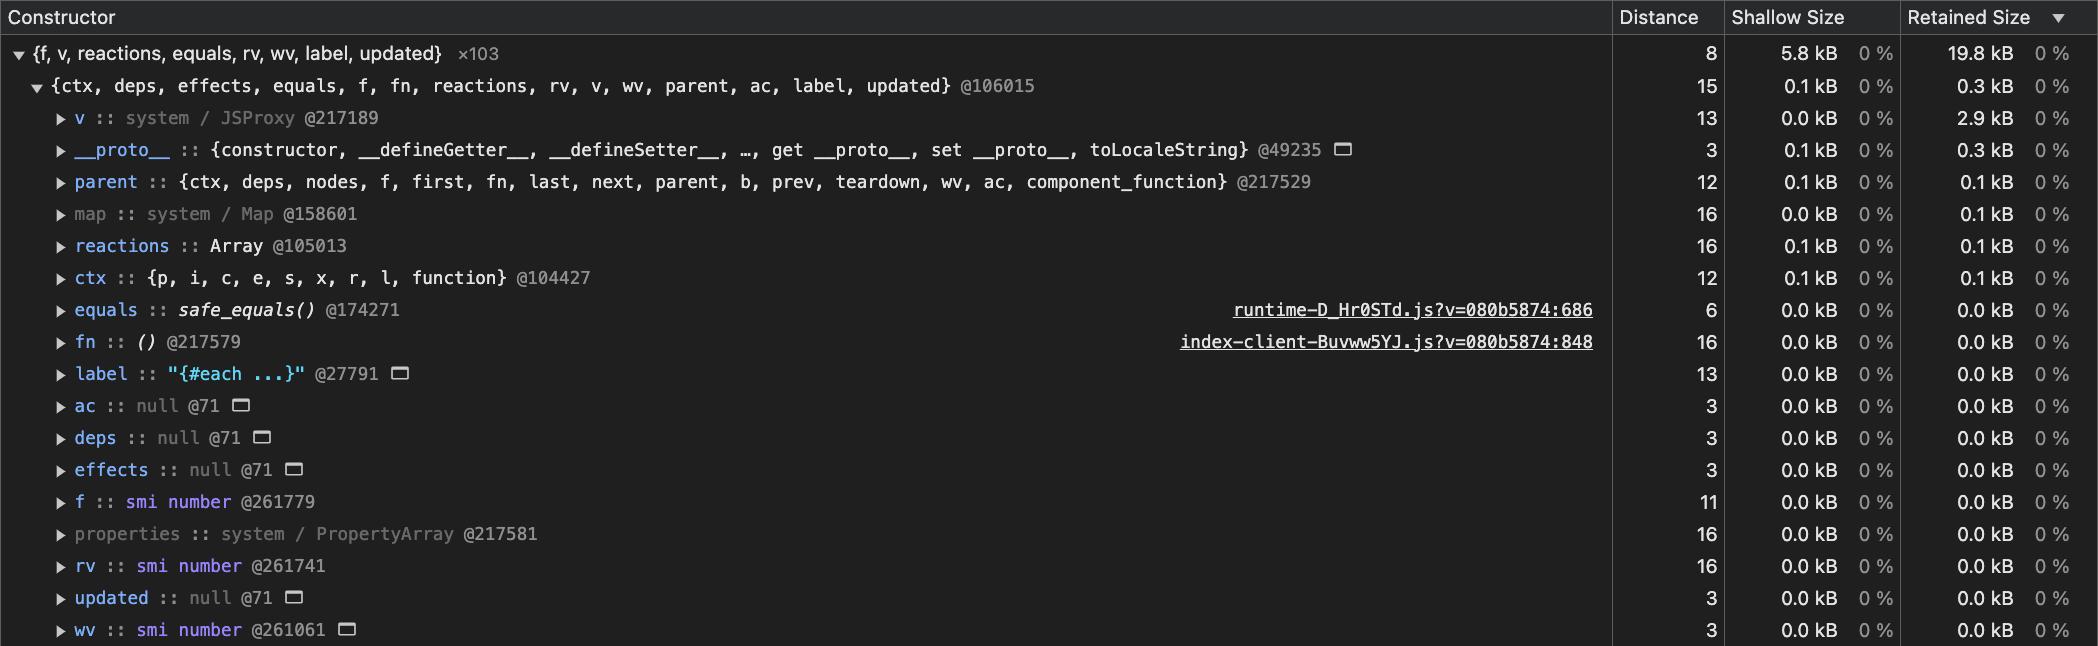
\includegraphics[width=\textwidth]{bilder/heap-svelte-signal}
    \subcaption{Svelte 5: Signal-POJO \texttt{\{f, v, reactions, \ldots\}}}
    \label{fig:heap-svelte}
  \end{subfigure}
  \caption[Chrome DevTools Heap-Snapshot ($n = 100$, Dev-Build): interne Objekte im Vergleich]{Chrome DevTools Heap-Snapshot ($n = 100$, Dev-Build):
           aufgeklappte interne Objekte beider Frameworks im Vergleich.
           Reacts \texttt{FiberNode} enthält neben Produktionsfeldern
           neun ausschließlich im Dev-Build vorhandene Debug-Felder
           (\texttt{\_debugStack}, \texttt{actualDuration} u.\,a.),
           während Sveltes Signal-POJO auf acht Felder beschränkt ist;
           die Feldanzahlen sind in (a) und (b) direkt ablesbar
           (Architekturkontext: \cref{sss:fiber-engine-structure,sss:runes-overhead}).}
  \label{fig:heap-structures}
\end{figure}

\newpage
\subsection{JS-Heap-Delta und Speicher-Overhead-Verhältnis}
\label{ss:results-h3-scaling}

Das JS-Heap-Delta $\Delta_{\mathrm{Heap}}$ wächst bei React über alle $n$-Stufen deutlich stärker als bei Svelte (\cref{fig:h3-memory}a). Beide Kurven steigen stetig mit~$n$. Der Abstand zwischen den Frameworks nimmt dabei mit zunehmendem $n$ zu. Der Frequenzeinfluss auf $\Delta_{\mathrm{Heap}}$ ist vernachlässigbar: Der React-Wert beträgt ca. $4450\,\text{kB}$ ($f = 10\,\text{Hz}$) bzw. ca. $4830\,\text{kB}$ ($f \approx 62\,\text{Hz}$) bei $n = 10\,000$. Der in \cref{fig:h3-memory}b gezeigte Speicher-Overhead-Faktor liegt bei $n = 100$ bei $2{,}8\times$ und erreicht bei $n = 6000$ ein Maximum von $6{,}4\times$. Dieser Anstieg lässt sich durch die in \cref{ss:results-h3-qualitative} ermittelte Retained Size der \texttt{FiberNode}-Instanzen erklären: React benötigt pro Komponenteninstanz erheblich mehr Speicher als Sveltes Signal-POJOs (vgl. \cref{sss:runes-overhead}). Auffällig ist, dass der Overhead-Faktor nach dem Maximum ($n = 6000$: $6{,}37\times$) nicht weiter ansteigt, sondern für größere $n$ wieder abnimmt ($n = 8000$: $6{,}24\times$, $n = 10\,000$: $6{,}18\times$; zuvor $n = 4000$: $5{,}92\times$). Diese Abflachung ab $n = 6000$ lässt sich anhand der vorliegenden Daten nicht eindeutig begründen und wird daher lediglich dokumentiert.
\begin{figure}[H]
  \centering
  \begin{minipage}[t]{\textwidth}
    \centering
    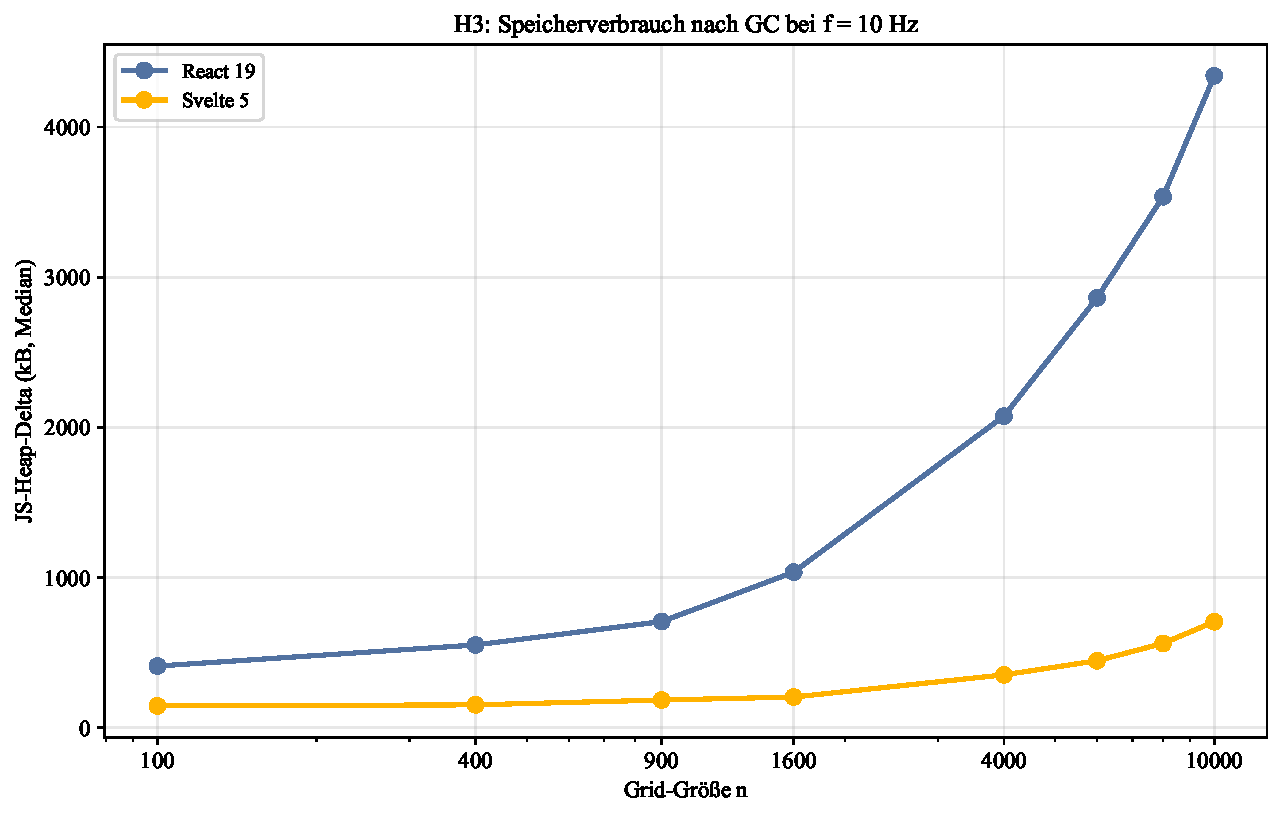
\includegraphics[width=\textwidth,keepaspectratio]{bilder/h3_memory}
    \subcaption{JS-Heap-Delta ($\Delta_{\mathrm{Heap}}$, in kB) bei $f = 10\,\text{Hz}$}
    \label{fig:h3-memory-abs}
  \end{minipage}
  \vspace{1.5em}
  \begin{minipage}[t]{\textwidth}
    \centering
    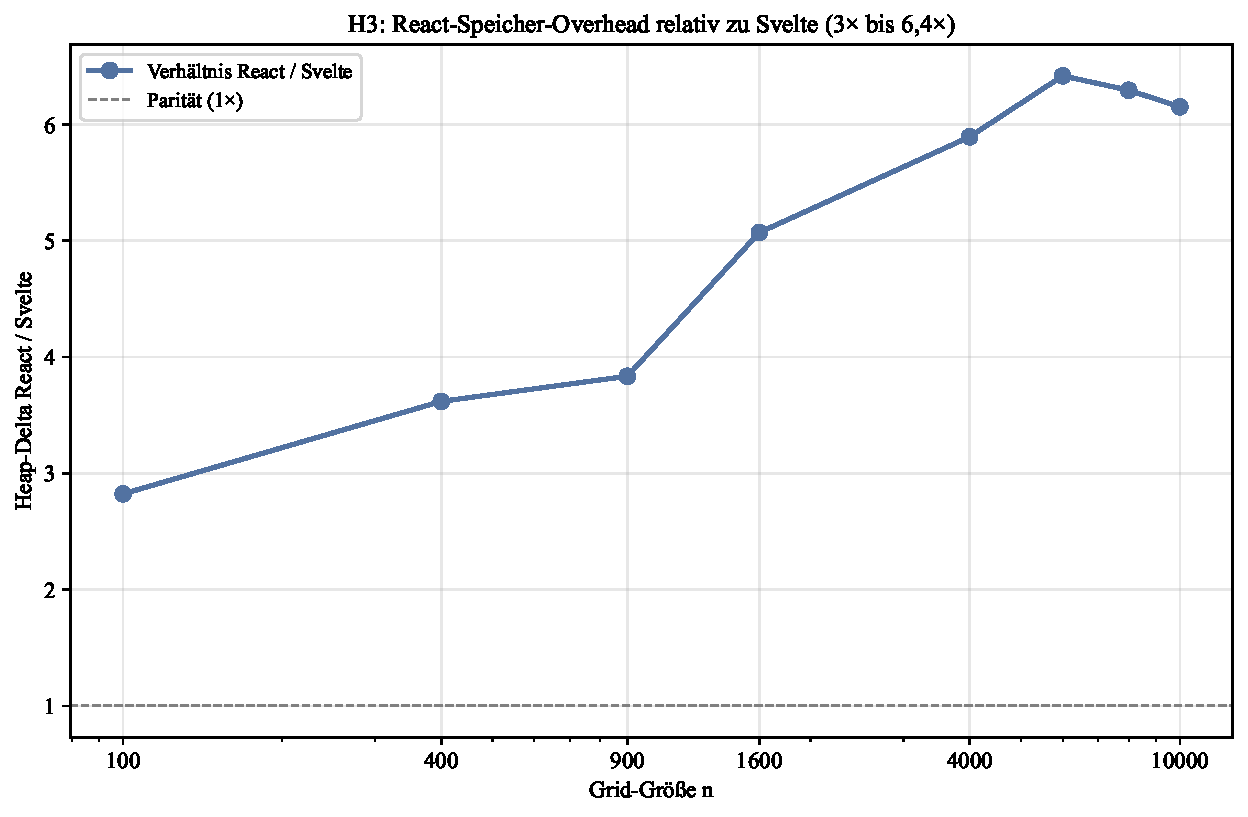
\includegraphics[width=\textwidth,keepaspectratio]{bilder/h3_memory_ratio}
    \subcaption{Speicher-Overhead-Faktor React\,/\,Svelte über $n$ bei $f = 10\,\text{Hz}$}
    \label{fig:h3-memory-ratio}
  \end{minipage}
  \caption[H3 – Speicherauswertung: JS-Heap-Delta beider Frameworks bei $f = 10\,\text{Hz}$]{H3 – Speicherauswertung: (a) medianes JS-Heap-Delta beider Frameworks
           bei $f = 10\,\text{Hz}$; (b) Quotient React\,/\,Svelte bei
           $f = 10\,\text{Hz}$ über alle $n$-Stufen (vgl.~\cref{ss:memory-efficiency}).}
  \label{fig:h3-memory}
\end{figure}

\subsection{Bewertung von H3}
\label{ss:results-h3-verdict}

H3 formuliert die Hypothese bezogen auf die Retained Size pro Komponente (\cref{ss:hypotheses}); diese ist in \cref{ss:results-h3-qualitative} qualitativ bestätigt: Bei $n = 100$ beträgt die Retained Size gesamt React $131\,\text{kB}$ vs. Svelte $19{,}8\,\text{kB}$ (vgl.~\cref{tab:heap-qualitative}), entspricht ${\approx}1{,}31\,\text{kB}$ vs. ${\approx}0{,}20\,\text{kB}$ pro Komponente: Faktor ${\approx}6{,}6\times$. Da der \texttt{FiberNode} im Development-Build neun zusätzliche Debug-Felder enthält (\cref{fig:heap-structures}), die im Production-Build nicht vorhanden sind, ist das gemessene Verhältnis gegenüber dem Production-Build nach oben verzerrt. Das JS-Heap-Delta $\Delta_{\mathrm{Heap}}$ misst die Skalierung quantitativ über alle $n$-Stufen im Production-Build (\cref{sss:quantitative-heap}) und bildet damit die belastbarere Vergleichsbasis für H3. React weist über alle $n$-Stufen einen deutlich höheren Speicherverbrauch auf als Svelte; der Overhead reicht von $2{,}8\times$ ($n = 100$) bis $6{,}4\times$ ($n = 6000$). Die Richtung dieses Faktors ist konsistent mit den im Development-Build beobachteten Unterschieden in der Retained Size der internen Datenstrukturen (\cref{ss:results-h3-qualitative}). Die dort ermittelten konkreten Verhältniswerte sind jedoch nicht direkt auf den Production-Build übertragbar. Die beobachtete Abflachung des Overhead-Faktors ab $n = 6000$ weicht zwar vom erwarteten Wachstum ab, steht jedoch nicht im Widerspruch zu H3. \textbf{H3 wird bestätigt.}

\section{H1: Interaktionslatenz (INP) unter Last}
\label{s:results-h1}

\subsection{INP-Verlauf über die Grid-Größe}
\label{ss:results-h1-curves}

\Cref{fig:h1-inp} zeigt den INP beider Frameworks bei $f = 10\,\text{Hz}$ und $f \approx 62\,\text{Hz}$ über alle $n$-Stufen. Der maximale gemessene INP beträgt $144\,\text{ms}$ (React, $n = 10\,000$, $f \approx 62\,\text{Hz}$) und liegt damit durchgängig im Bereich „Good" ($\leq 200\,\text{ms}$) der Web-Vitals-Klassifikation (\cref{ss:inp}). Dennoch steigt der INP beider Frameworks mit wachsender UI-Dichte spürbar an; React erreicht in der Mehrzahl der Szenarien höhere Werte als Svelte.
\begin{figure}[H]
  \centering
  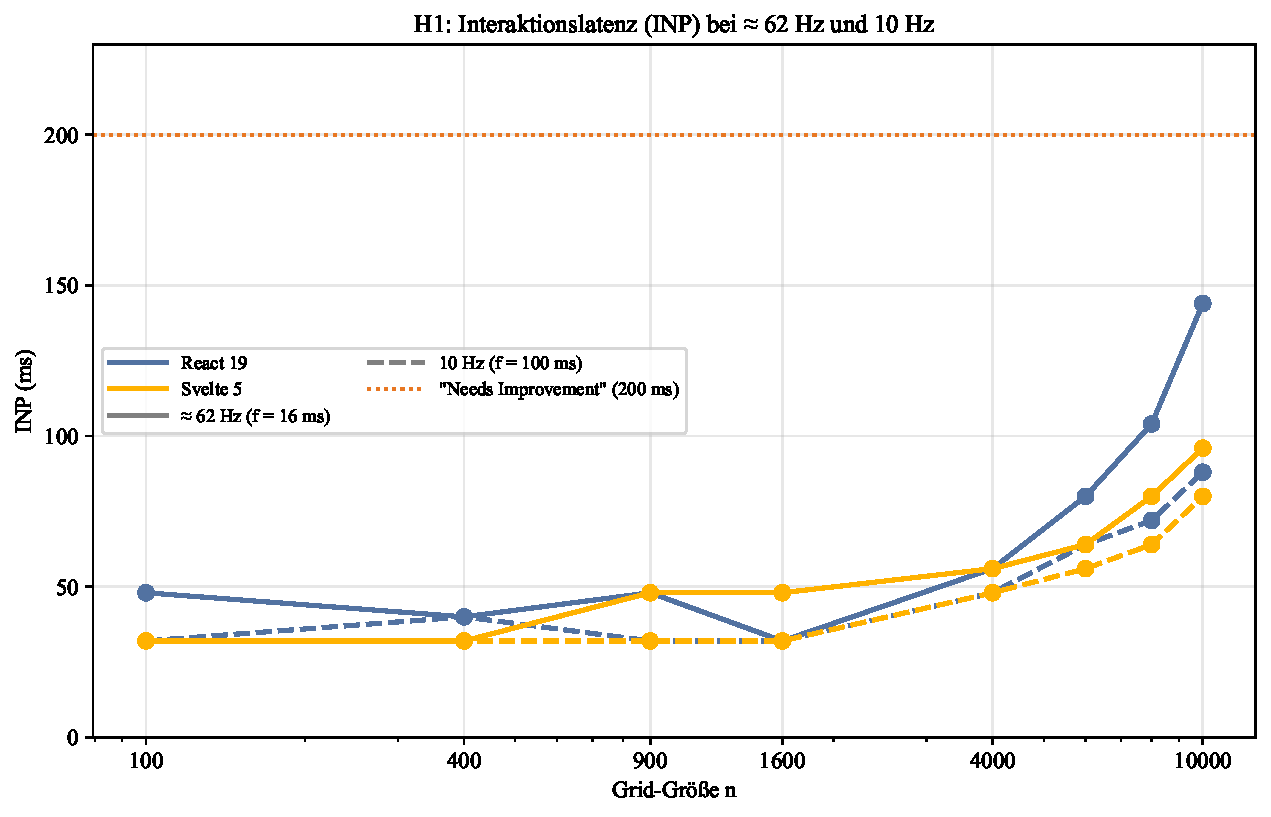
\includegraphics[width=\textwidth,keepaspectratio]{bilder/h1_inp}
  \caption[H1 – INP beider Frameworks bei $f \approx 62\,\text{Hz}$ und $f = 10\,\text{Hz}$ über alle $n$-Stufen]{H1 – INP beider Frameworks bei $f \approx 62\,\text{Hz}$ und $f = 10\,\text{Hz}$
           über alle $n$-Stufen (\cref{ss:inp}).}
  \label{fig:h1-inp}
\end{figure}

\subsection{Zerlegung der INP-Phasen}
\label{ss:results-h1-phases}

\Cref{tab:inp-phases} teilt die INP-Komponenten \textit{inputDelay} (iD), \textit{processingTime} (pT) und \textit{presentationDelay} (pD) für ausgewählte Szenarien auf und zeigt, in welcher Phase die Latenz entsteht (\cref{ss:inp}). Die \textit{processingTime} trägt in keinem Szenario wesentlich zum INP bei: Sie überschreitet $1{,}0\,\text{ms}$ bei React nicht (Maximum: $n = 4000$, $f = 20\,\text{Hz}$) und beträgt für Svelte selbst unter Extremlast ($n = 10\,000$, $f \approx 62\,\text{Hz}$) lediglich $0{,}7\,\text{ms}$. Die INP-Verschlechterung mit steigendem~$n$ wird damit ausschließlich durch \textit{inputDelay} (blockierter Main Thread) und \textit{presentationDelay} (Rendering nach dem Handler) bestimmt. Wie sich die Latenz auf diese beiden Phasen verteilt, hängt von der Last ab (\cref{tab:inp-phases}). Bei niedriger Last ($n \leq 1600$) macht die \textit{presentationDelay} den größten Anteil aus: Bei React, $n = 100$, $f = 10\,\text{Hz}$ beträgt der \textit{inputDelay} lediglich $0{,}4\,\text{ms}$, während die \textit{presentationDelay} $31{,}5\,\text{ms}$ ausmacht. Bei hoher UI-Dichte und niedriger Frequenz ($n = 10\,000$, $f = 10\,\text{Hz}$) bleibt die \textit{presentationDelay} zwar der größte Anteil ($51{,}9\,\text{ms}$), der \textit{inputDelay} wächst jedoch auf $36{,}1\,\text{ms}$ an und trägt damit spürbar zum INP bei. Unter Extremlast kann der \textit{inputDelay} die \textit{presentationDelay} schließlich überschreiten: Bei React, $n = 8000$, $f \approx 62\,\text{Hz}$ beträgt er $69{,}6\,\text{ms}$ gegenüber $34{,}4\,\text{ms}$. In nahezu allen Szenarien überwiegt die \textit{presentationDelay} weiterhin; die beschriebene Ausnahme bleibt auf dieses eine Szenario beschränkt. Hauptursache des wachsenden \textit{inputDelay} sind die in \cref{s:results-h2} gemessenen Scripting-Kosten, die den Main Thread blockieren. Szenariospezifische Besonderheiten werden nachfolgend diskutiert. Eine Ausnahme zeigt jedoch, dass ein niedrigerer Scripting-Aufwand nicht automatisch zu einem besseren INP führt (\cref{tab:inp-phases}, unterer Abschnitt). 

\noindent\textbf{Ausnahme\,1} ($n = 10\,000$, $f = 20\,\text{Hz}$): React erzielt einen INP von $96\,\text{ms}$ (iD: $20{,}9\,\text{ms}$; pT: $0\,\text{ms}$; pD: $75{,}1\,\text{ms}$), Svelte einen INP von $104\,\text{ms}$ (iD: $18{,}0\,\text{ms}$; pT: $0\,\text{ms}$; pD: $86{,}0\,\text{ms}$). Svelte weist sowohl geringere Scripting-Kosten als auch einen niedrigeren \textit{inputDelay} auf und erzielt dennoch den höheren INP. Die Ursache liegt in der \textit{presentationDelay} ($86{,}0\,\text{ms}$ vs. $75{,}1\,\text{ms}$). Sveltes höhere Rendering-Zeit bei $f = 20\,\text{Hz}$ ($13{,}71\,\text{ms}$ vs. $11{,}87\,\text{ms}$, vgl. \cref{ss:results-h2-scripting}) spricht für dieselbe Ursache, erklärt quantitativ jedoch nur einen Teil des \textit{presentationDelay}-Unterschieds von $10{,}9\,\text{ms}$. Der genaue Mechanismus der verbleibenden Differenz lässt sich anhand der vorliegenden Daten nicht bestimmen. Das zeigt: Geringere Scripting-Kosten garantieren keinen besseren INP; der Rendering-Nachteil kann den Scripting-Vorteil überwiegen. Daneben bestätigt die Phasenzerlegung einen zweiten Aspekt von H1 unmittelbar (\cref{tab:inp-phases}). 

\noindent\textbf{H1-Bestätigung} ($n = 1600$, $f \geq 30\,\text{Hz}$): Bei $\Delta t = 16\,\text{ms}$ beträgt der INP für React $32\,\text{ms}$ (iD: $5{,}5\,\text{ms}$; pT: $0{,}1\,\text{ms}$; pD: $26{,}4\,\text{ms}$), für Svelte hingegen $48\,\text{ms}$ (iD: $4{,}6\,\text{ms}$; pT: $0\,\text{ms}$; pD: $43{,}4\,\text{ms}$). Bei $\Delta t = 33\,\text{ms}$ gilt dasselbe: React $32\,\text{ms}$ (iD: $6{,}7\,\text{ms}$; pT: $0{,}2\,\text{ms}$; pD: $25{,}1\,\text{ms}$) gegenüber Svelte $40\,\text{ms}$ (iD: $4{,}5\,\text{ms}$; pT: $0\,\text{ms}$; pD: $35{,}5\,\text{ms}$). In diesen Szenarien liegen die Scripting- und Rendering-Kosten beider Frameworks auf einem niedrigen Wert (Scripting: $0{,}75$--$1{,}61\,\text{ms}$/Tick; Rendering: $1{,}73$--$1{,}91\,\text{ms}$/Tick); die Rendering-Zeiten sind dabei nahezu gleich ($f \approx 62\,\text{Hz}$: $1{,}75$ vs. $1{,}73\,\text{ms}$/Tick; $f \approx 30\,\text{Hz}$: $1{,}91$ vs. $1{,}87\,\text{ms}$/Tick). Svelte weist bei beiden Frequenzstufen den niedrigeren \textit{inputDelay} auf ($4{,}6\,\text{ms}$ bzw.\ $4{,}5\,\text{ms}$ gegenüber $5{,}5\,\text{ms}$ bzw.\ $6{,}7\,\text{ms}$ bei React). Dennoch überwiegt der Unterschied in der \textit{presentationDelay} im Gesamtergebnis: Er beträgt $17{,}0\,\text{ms}$ ($f \approx 62\,\text{Hz}$) bzw.\ $10{,}4\,\text{ms}$ ($f \approx 30\,\text{Hz}$) zugunsten Reacts und bestimmt damit den höheren INP von Svelte. Die Ursache dieses pD-Unterschieds unterscheidet sich von Ausnahme\,1: Dort lag sie in Sveltes höherer Rendering-Zeit. Hier sind die Rendering-Zeiten nahezu identisch, sodass ein Scheduling-Effekt als Erklärung naheliegt. Als mögliche Ursache kommt Reacts prioritätsbasiertes Scheduling infrage, das Klick-Events gegenüber Hintergrund-Updates priorisiert, während Sveltes synchrones Effect-Batching vergleichbare Priorisierungsmöglichkeiten nicht vorsieht (\cref{sss:scheduling-priotising-of-updates,sss:microtasks}); der genaue Mechanismus lässt sich anhand der vorliegenden Daten nicht bestimmen. Dieser Scheduling-Vorteil Reacts tritt ausschließlich ab $f \geq 30\,\text{Hz}$ auf; bei $n = 1600$ und $f = 10\,\text{Hz}$ sowie $f = 20\,\text{Hz}$ sind die INP-Werte beider Frameworks gleich ($32\,\text{ms}$, vgl.~\cref{tab:appendix-benchmark}). Dieses Ergebnis ist konsistent mit H1: Bei Last unterhalb des Frame-Budgets stabilisiert Reacts Scheduling den INP, auch wenn die absoluten Scripting-Kosten höher sind — bei $n = 1600$ und $f \approx 62\,\text{Hz}$ beträgt der INP-Vorteil $16\,\text{ms}$ (React $32\,\text{ms}$ vs.\ Svelte $48\,\text{ms}$, $+50\,\%$) — ein Scheduling-Vorteil, kein Effizienz-Vorteil.

\noindent\textbf{Ausnahme\,2} ($n = 10\,000$, $f \approx 30\,\text{Hz}$, \cref{tab:inp-phases}) bildet eine weitere, durch H1 nicht abgedeckte Einschränkung: Beide Frameworks erzielen denselben INP ($104\,\text{ms}$), jedoch mit gegenläufiger Phasenverteilung. React weist einen \textit{inputDelay} von $5\,\text{ms}$ auf, was mit dem in der H1-Bestätigung beschriebenen Scheduling-Vorteil konsistent ist (\cref{sss:scheduling-priotising-of-updates}), während Sveltes \textit{inputDelay} $51{,}8\,\text{ms}$ beträgt (der höchste Svelte-Wert im gesamten Datensatz). Eine \textit{presentationDelay} von $99\,\text{ms}$ hebt diesen Vorteil jedoch vollständig auf. Bei einer Rendering-Zeit von $8{,}40\,\text{ms}$/Tick entspricht dies der höchsten React-\textit{presentationDelay} im Datensatz, deren Ursache sich mit den erhobenen Metriken nicht eindeutig bestimmen lässt (vgl.~\cref{s:limitations}). Der Gleichstand ergibt sich damit als Überlagerung des Scheduling-Vorteils Reacts mit einem ungeklärten \textit{presentationDelay}-Ausreißer; kein Widerspruch zu H1, aber eine weitere Einschränkung.
\begin{table}[H]
  \centering
  \caption[INP-Phasenzerlegung für ausgewählte Szenarien]{INP-Phasenzerlegung für ausgewählte Szenarien (Datenquelle:
           \texttt{summary.csv}, vgl.~\cref{ss:impl-results})}
  \label{tab:inp-phases}
  \small
  \begin{tabular}{llrrrrr}
    \toprule
    \textbf{Framework} & \textbf{Szenario}
      & \textbf{INP} & \textbf{iD} & \textbf{pT} & \textbf{pD}
      & \textbf{Scripting} \\
    & ($n$\,/\,$f$)
      & (ms) & (ms) & (ms) & (ms)
      & (ms/Tick) \\
    \midrule
    \multicolumn{7}{l}{\textit{Niedrige Last (pD-bestimmt)}} \\
    React  & 100\,/\,$10\,\text{Hz}$
      & 32  & 0{,}4  & 0{,}1 & 31{,}5 & 0{,}27 \\
    \midrule
    \multicolumn{7}{l}{\textit{Hohe Last (iD wächst)}} \\
    React  & 10\,000\,/\,$10\,\text{Hz}$
      & 88  & 36{,}1 & 0{,}0 & 51{,}9 & 11{,}24 \\
    Svelte & 10\,000\,/\,$10\,\text{Hz}$
      & 80  & 1{,}9  & 0{,}0 & 78{,}1 & 4{,}12 \\
    \midrule
    \multicolumn{7}{l}{\textit{Extremlast (iD $>$ pD)}} \\
    React  & 8\,000\,/\,${\approx}\,62\,\text{Hz}$
      & 104 & 69{,}6 & 0{,}0 & 34{,}4 & 3{,}53 \\
    Svelte & 8\,000\,/\,${\approx}\,62\,\text{Hz}$
      & 80  & 32{,}1 & 0{,}0 & 47{,}9 & 3{,}08 \\
    \midrule
    \multicolumn{7}{l}{\textit{Ausnahme\,1: Svelte-INP $>$ React trotz niedrigerem iD}} \\
    React  & 10\,000\,/\,$20\,\text{Hz}$
      & 96  & 20{,}9 & 0{,}0 & 75{,}1 & 11{,}17 \\
    Svelte & 10\,000\,/\,$20\,\text{Hz}$
      & 104 & 18{,}0 & 0{,}0 & 86{,}0 & 4{,}29 \\
    \midrule
    \multicolumn{7}{l}{\textit{H1-Bestätigung: Scheduling-Vorteil React bei $n = 1600$, $f \geq 30\,\text{Hz}$}} \\
    React  & 1\,600\,/\,${\approx}\,62\,\text{Hz}$
      & 32  & 5{,}5  & 0{,}1 & 26{,}4 & 1{,}57 \\
    Svelte & 1\,600\,/\,${\approx}\,62\,\text{Hz}$
      & 48  & 4{,}6  & 0{,}0 & 43{,}4 & 0{,}75 \\
    React  & 1\,600\,/\,${\approx}\,30\,\text{Hz}$
      & 32  & 6{,}7  & 0{,}2 & 25{,}1 & 1{,}61 \\
    Svelte & 1\,600\,/\,${\approx}\,30\,\text{Hz}$
      & 40  & 4{,}5  & 0{,}0 & 35{,}5 & 0{,}76 \\
    \midrule
    \multicolumn{7}{l}{\textit{Ausnahme\,2: Gleichstand trotz gegenläufiger Phasenverteilung}} \\
    React  & 10\,000\,/\,${\approx}\,30\,\text{Hz}$
      & 104 & 5{,}0  & 0{,}0 & 99{,}0 & 7{,}43 \\
    Svelte & 10\,000\,/\,${\approx}\,30\,\text{Hz}$
      & 104 & 51{,}8 & 0{,}0 & 52{,}2 & 4{,}09 \\
    \bottomrule
  \end{tabular}
\end{table}

\subsection{Bewertung von H1}
\label{ss:results-h1-verdict}

Über alle vier Frequenzstufen hinweg weist Svelte bei hoher UI-Dichte ($n \geq 4000$) in zwölf von 16~Szenarien einen niedrigeren INP auf als React. In zwei weiteren Szenarien ($n = 4000$, $f = 10\,\text{Hz}$ und $f \approx 62\,\text{Hz}$) sind die INP-Werte beider Frameworks gleich ($48\,\text{ms}$ bzw.\ $56\,\text{ms}$). Der in H1 erwartete Svelte-Vorteil bei hoher Dichte (\cref{ss:hypotheses}) zeigt sich durch die höheren Scripting-Kosten von React (\cref{s:results-h2}), die primär den \textit{inputDelay} erhöhen ($n = 10\,000$, $f = 10\,\text{Hz}$: $36{,}1\,\text{ms}$ gegenüber $1{,}9\,\text{ms}$ bei Svelte). Anzumerken ist, dass bei $n = 10\,000$ und $f \approx 62\,\text{Hz}$ (dem Szenario mit dem größten INP-Abstand, $96\,\text{ms}$ vs.\ $144\,\text{ms}$) Svelte trotz geringfügig höherer Scripting-Zeit ($3{,}66\,\text{ms}$ vs.\ $3{,}42\,\text{ms}$, vgl.~\cref{ss:results-h2-scripting}) einen niedrigeren \textit{inputDelay} aufweist ($34{,}1\,\text{ms}$ vs.\ $56{,}9\,\text{ms}$). Der direkte Kausalzusammenhang Scripting\,$\rightarrow$\,\textit{inputDelay} greift bei $f \approx 62\,\text{Hz}$ somit nicht; dies deutet auf frequenzabhängige Scheduling-Effekte hin. Bei niedriger Dichte weist Svelte ebenfalls niedrigere INP-Werte auf: bei $n = 100$ ausschließlich bei $f \approx 62\,\text{Hz}$ ($32\,\text{ms}$ vs.\ $48\,\text{ms}$), bei $n = 400$ sowohl bei $f \approx 62\,\text{Hz}$ als auch bei $f = 10\,\text{Hz}$ (jeweils $32\,\text{ms}$ vs.\ $40\,\text{ms}$). In allen diesen Fällen resultiert der Unterschied ausschließlich aus der \textit{presentationDelay}, da die Scripting-Kosten auf diesen Stufen vernachlässigbar sind. Der in H1 ebenfalls vorhergesagte Scheduling-Vorteil Reacts bei Last unterhalb des Frame-Budgets bestätigt sich bei $n = 1600$ und $f \geq 30\,\text{Hz}$ (vgl.~\cref{ss:results-h1-phases}). Zwei Szenarien, in denen die \textit{presentationDelay} das durch H1 vorhergesagte INP-Ergebnis überlagert, schränken die Gesamtaussage ein: Bei $n = 10\,000$ und $f = 20\,\text{Hz}$ übersteigt Sveltes INP den von React infolge einer höheren \textit{presentationDelay} durch Rendering-Bündelung (\cref{ss:results-h1-phases}). Bei $n = 10\,000$ und $f \approx 30\,\text{Hz}$ ergibt sich ein Gleichstand mit gegenläufiger, ungeklärter Phasenverteilung (\cref{ss:results-h1-phases}). Da der Svelte-Vorteil in der deutlichen Mehrheit der Szenarien bei $n \geq 4000$ gilt und beide Teilaussagen von H1 empirisch bestätigt sind, stützen die Befunde H1 trotz dieser Einschränkungen. \textbf{H1 wird bestätigt.}

\section{H4: Identifikation des Tipping Points}
\label{s:results-h4}

Während H2 beschreibt, wie stark der Scripting-Aufwand mit $n$ wächst, fragt H4, ab welchem $n$ das Frame-Budget überschritten wird und welches Framework diesen Tipping Point zuerst erreicht (\cref{ss:hypotheses}).

\subsection{Frame-Budget-Auslastung und Long Tasks}
\label{ss:results-h4-tipping}

\Cref{fig:h4-tipping}a zeigt, bei welchem $n$ die kombinierte Summe aus Scripting- und Rendering-Zeit die $16{,}7\,\text{ms}$-Grenze des Frame-Budgets bei $f = 20\,\text{Hz}$ überschreitet. React erreicht diesen Schwellenwert bei einer niedrigeren UI-Dichte als Svelte. Dies bestätigt die Vorhersage aus \cref{sss:tipping-point}: Die Abstraktionskosten der Fiber-Architektur führen dazu, dass der Main Thread bei React früher vollständig ausgelastet ist als bei Svelte mit seiner feingranularen Reaktivität.
Zu beachten ist, dass die $16{,}7\,\text{ms}$-Grenze als Frame-Budget nur dann direkt relevant ist, wenn Tick-Intervall und Framelänge übereinstimmen ($f \approx 62\,\text{Hz}$). Bei niedrigeren Frequenzen bedeutet eine Überschreitung dieser Grenze nicht zwingend einen Frame-Drop, da der Main Thread zwischen den Ticks ausreichend Zeit für das Rendering hat (\cref{sss:frame-budget}). Die Anzahl der Long Tasks (\cref{fig:h4-tipping}b) bestätigt dies bei niedrigen bis mittleren Frequenzen, zeigt jedoch bei $f \approx 62\,\text{Hz}$ eine Umkehr des Long-Task-Verhältnisses. Bei $f \approx 30\,\text{Hz}$ und $n = 10\,000$ erzeugt React rund $45$ Long Tasks, Svelte $22{,}5$. Die IQR-Streuung ist dabei hoch (React: $27$, Svelte: $28$; aus Rohdaten, nicht in \cref{tab:appendix-benchmark}); bei Svelte übersteigt der IQR sogar den Median, was die Aussagekraft dieses Vergleichs einschränkt. Ab $f \approx 62\,\text{Hz}$ dreht sich das Verhältnis: Svelte erzeugt $91$ Long Tasks gegenüber $86$ bei React. Diese Umkehrung tritt ausschließlich bei $n = 10\,000$ auf; bei $n = 8000$ und $f \approx 62\,\text{Hz}$ hat React mit $58$ Long Tasks weiterhin deutlich mehr als Svelte mit $29$. Es handelt sich somit nicht um ein generelles Muster, sondern um einen Extremlast-Effekt: Bei $f \approx 62\,\text{Hz}$ stapelt Sveltes synchrones Effect-Batching (\cref{sss:microtasks,sss:scheduling-priotising-of-updates}) Arbeit ohne zwischenzeitliches Yielding, was zu einem überproportionalen Anstieg der Long Tasks führt (Svelte: $+\!304\,\%$; React: $+\!91\,\%$). Der Scripting-Schnittpunkt (\cref{ss:results-h2-scripting}) tritt im selben Szenario auf und ist konsistent mit diesem Befund.
\begin{figure}[H]
  \centering
  \begin{minipage}[t]{\textwidth}
    \centering
    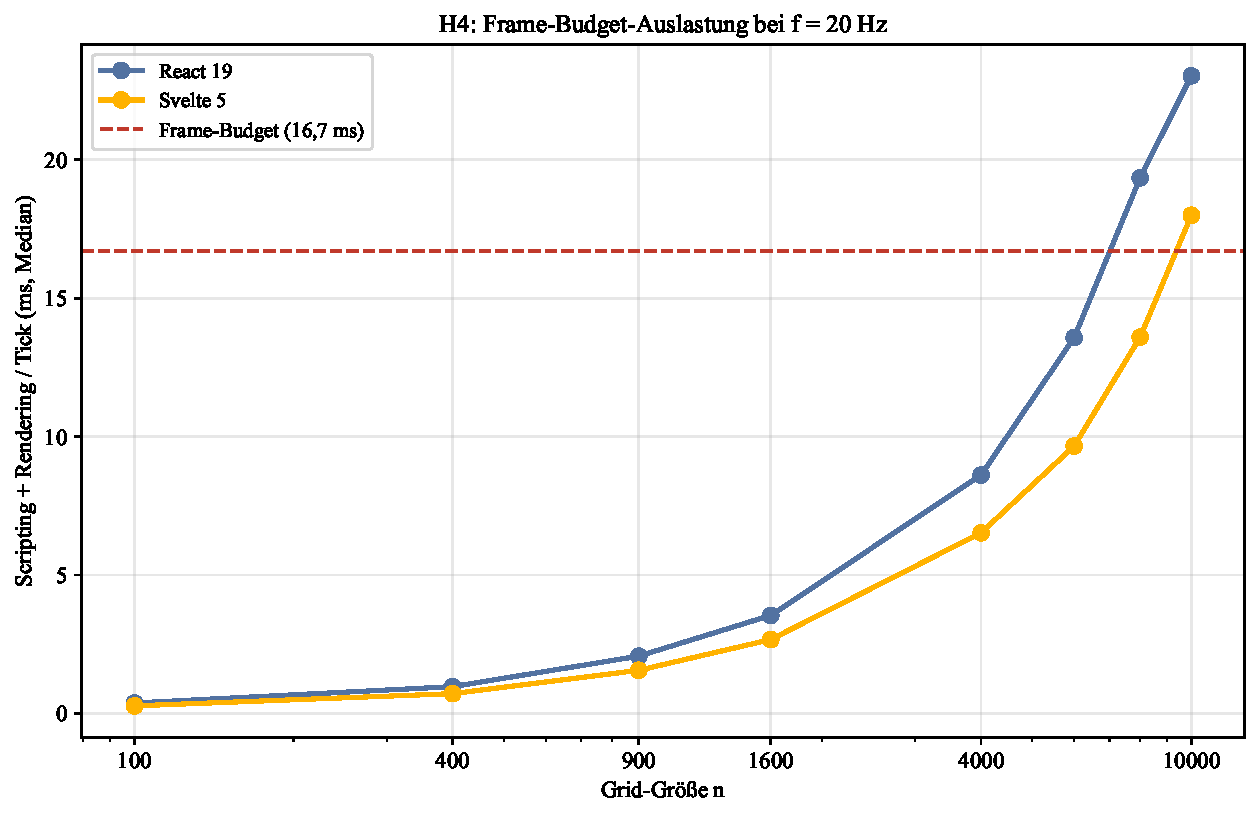
\includegraphics[width=\textwidth,keepaspectratio]{bilder/h4_frame_budget}
    \subcaption{(Scripting + Rendering) vs. $16{,}7\,\text{ms}$-Grenze bei $f = 20\,\text{Hz}$}
    \label{fig:h4-budget}
  \end{minipage}
  \vspace{0.75em}
  \begin{minipage}[t]{\textwidth}
    \centering
    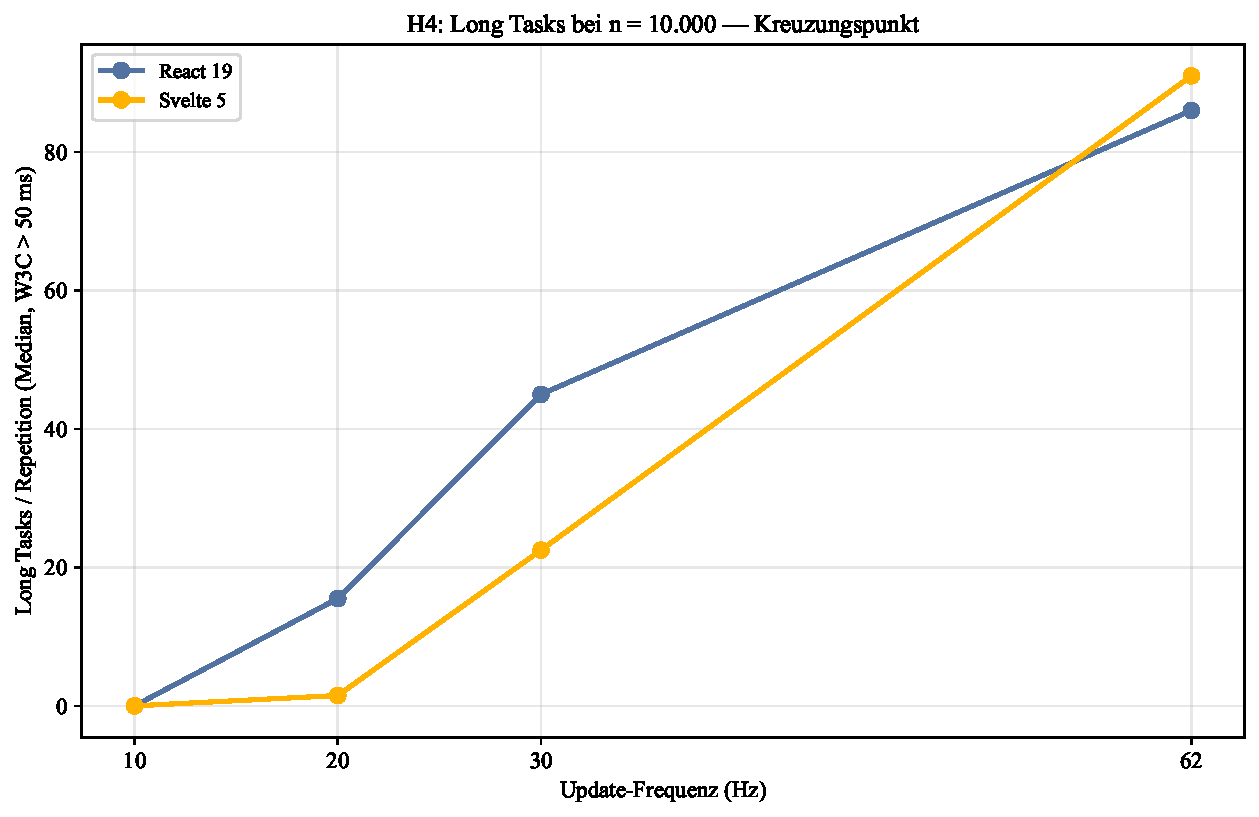
\includegraphics[width=\textwidth,keepaspectratio]{bilder/h4_long_tasks}
    \subcaption{Long Tasks bei $n = 10\,000$ über alle Frequenzstufen}
    \label{fig:h4-longtasks}
  \end{minipage}
  \caption[H4 – Tipping-Point-Analyse: Frame-Budget-Auslastung und Long Tasks]{H4 – Tipping-Point-Analyse: (a) Frame-Budget-Auslastung beider Frameworks
           bei $f = 20\,\text{Hz}$ mit $16{,}7\,\text{ms}$-Grenze; (b) Anzahl der Long Tasks bei $n = 10\,000$
           in Abhängigkeit von $f$
           (vgl.~\cref{sss:frame-budget,sss:long-task-measurement}).}
  \label{fig:h4-tipping}
\end{figure}

\subsection{Bewertung von H4}
\label{ss:results-h4-verdict}

Die Frame-Budget-Auswertung bestätigt die Hauptvorhersage von H4: React überschreitet die $16{,}7\,\text{ms}$-Grenze bei niedrigerer UI-Dichte als Svelte (\cref{sss:tipping-point}). Bei $f = 10\,\text{Hz}$ überschreitet React die Grenze ab $n = 8000$ ($19{,}59\,\text{ms}$), Svelte erst ab $n = 10\,000$ ($17{,}67\,\text{ms}$); bei $f = 20\,\text{Hz}$ zeigt sich dasselbe Muster: React ab $n = 8000$ ($19{,}35\,\text{ms}$), Svelte ab $n = 10\,000$ ($18{,}00\,\text{ms}$). Diese Grenzüberschreitung pro Tick tritt ausschließlich bei $f \leq 20\,\text{Hz}$ auf. Die konkret ermittelten $n$-Schwellenwerte sind V8\slash Chromium-spezifisch; andere JavaScript-Engines könnten den Tipping Point bei abweichenden $n$-/$f$-Kombinationen aufweisen (vgl.~\cref{s:limitations}). Bei $f \approx 30\,\text{Hz}$ erreicht die kombinierte Scripting- und Rendering-Zeit für React maximal $15{,}83\,\text{ms}$ ($n = 10\,000$: $7{,}43 + 8{,}40\,\text{ms}$), bei $f \approx 62\,\text{Hz}$ lediglich $8{,}37\,\text{ms}$ ($3{,}42 + 4{,}95\,\text{ms}$), jeweils unterhalb der Schwelle (vgl.~\cref{tab:appendix-benchmark}). Die Long-Task-Analyse zeigt bei $n = 10\,000$ und $f \approx 62\,\text{Hz}$ eine Umkehr des Long-Task-Verhältnisses (Svelte $91$ vs. React $86$ Long Tasks). Diese Umkehr belegt empirisch die in H4 vorhergesagte mögliche Rangfolge-Umkehr bei extremer Last (\cref{sss:tipping-point}). \textbf{H4 wird bestätigt.}

\section{Zusammenfassung der Ergebnisse}
\label{s:results-summary}

\Cref{tab:hypotheses-summary} fasst die Bewertungen der vier Hypothesen zusammen. H2 und H3 erklären die Befunde von H1 und H4: Die in H2 gemessenen Scripting-Kosten der Fiber-Architektur (\cref{s:results-h2}) begründen, warum React in H1 früher INP-Verschlechterungen zeigt (\cref{s:results-h1}) und in H4 das Frame-Budget bei niedrigerer UI-Dichte überschreitet (\cref{s:results-h4}). Die in H3 gemessenen Heap-Delta-Unterschiede (\cref{s:results-h3}) belegen, dass die zusätzlichen Abstraktionskosten nicht nur die CPU, sondern auch den Speicher belasten. H4 baut auf den CPU-Kurven aus H2 auf, wertet diese schwellenwertbasiert aus und bestimmt damit den Übergang vom kontrollierten Skalierungsbereich zur Main-Thread-Blockierung.
\begin{table}[H]
  \centering
  \caption{Zusammenfassung der Hypothesenbewertungen (H1–H4)}
  \label{tab:hypotheses-summary}
  \small
  \begin{tabular}{llp{7.5cm}}
    \toprule
    \textbf{Hypothese} & \textbf{Ergebnis} & \textbf{Kernaussage} \\
    \midrule
    H1 & bestätigt &
      Svelte erzielt bei $n \geq 4000$ in der Mehrzahl der Szenarien niedrigere
      INP-Werte; Reacts Scheduling-Vorteil zeigt sich erwartungsgemäß bei
      $n = 1600\,/\,{\geq}30\,\text{Hz}$; ungeklärte Ausnahmen bei
      $n = 10\,000\,/\,20\,\text{Hz}$ (Svelte schlechter) und
      $n = 10\,000\,/\,30\,\text{Hz}$ (Gleichstand). \\[4pt]
    H2 & teilweise bestätigt &
      Reacts Scripting-Aufwand pro Tick wächst bei $f \leq 30\,\text{Hz}$ stärker
      als Sveltes; bei $f \approx 62\,\text{Hz}$ und $n = 10\,000$ tritt
      ein Scripting-Schnittpunkt auf (Svelte $3{,}66\,\text{ms}$ vs. React $3{,}42\,\text{ms}$). \\[4pt]
    H3 & bestätigt &
      Qualitativ bestätigt durch Retained Size: React $131\,\text{kB}$
      vs.\ Svelte $19{,}8\,\text{kB}$ (${\approx}1310$ vs.\ ${\approx}198$\,B
      pro Komponente) bei $n = 100$ im Dev-Build
      (vgl.~\cref{tab:heap-qualitative}); quantitativ im Production-Build:
      Heap-Delta-Faktor $2{,}8\times$ ($n = 100$) bis $6{,}4\times$
      ($n = 6000$), danach leicht rückläufig. \\[4pt]
    H4 & bestätigt &
      React überschreitet das $16{,}7\,\text{ms}$-Frame-Budget bei
      niedrigerem $n$ als Svelte; bei $n = 10\,000\,/\,62\,\text{Hz}$
      erzeugt Svelte mehr Long Tasks ($91$ vs.~$86$). \\
    \bottomrule
  \end{tabular}
\end{table}

\section{Limitationen}
\label{s:limitations}

Die folgenden Einschränkungen betreffen die Interpretierbarkeit der konkreten Befunde und ergänzen die in \cref{ss:external-validity} diskutierte externe Validität des Versuchsdesigns.

\subsection{Fehlende Isolation des Compiler-Einflusses}
React~19 wurde ausschließlich mit aktiviertem Compiler gemessen. Der Compiler lässt das komponentenbasierte Render-Modell und die Fiber-Architektur unverändert; die Reconciliation wird weiterhin ausgeführt (\cref{sss:potentials-and-limitations}). Daher lässt sich im gewählten Versuchsaufbau nicht bestimmen, welcher Anteil der gemessenen Scripting-Kosten auf die Compiler-Memoisierung und welcher auf die VDOM-Reconciliation entfällt. Ein Test ohne Compiler hätte diesen Einfluss isolierbar gemacht, hätte jedoch die praktische Vergleichbarkeit beeinträchtigt, da Sveltes Vorteile ebenfalls durch Compile-Time-Optimierung entstehen (\cref{ss:svelte-compiler}).

\subsection{Ausschließlich Chromium}
Alle Messungen basieren auf Playwrights Chromium-Instanz mit V8 als JavaScript-Engine. Da die Messergebnisse das JIT-Verhalten von V8 widerspiegeln (\cref{sss:jit-interference}), könnten andere Engines — SpiderMonkey (Firefox) und JavaScriptCore (Safari) — den Tipping Point bei anderen $n$-/$f$-Kombinationen aufweisen. Die Ergebnisse gelten daher primär für Chromium-basierte Umgebungen.

\subsection{Verbleibende Browser-interne Störeinflüsse}
Trotz der in \cref{sss:gc-interference,sss:jit-interference} beschriebenen Vorkehrungen lassen sich Garbage-Collection-Pausen und JIT-Effekte nicht vollständig ausschließen. Der ungleichmäßige Scripting-Rückgang bei höherer Tick-Frequenz (\cref{ss:results-h2-scripting}) ist ohne V8-internes Profiling nicht eindeutig erklärbar und wurde daher im vorliegenden Kapitel als Spekulation gekennzeichnet.

\subsection{Presentationdelay als zusammengesetzte Metrik}
Die \textit{presentationDelay} erfasst die Zeit nach Abschluss der Skriptausführung bis zur sichtbaren Darstellung der Änderungen als einzelne Kennzahl (\cref{ss:inp}). Eine Zerlegung in Browser-interne Teilphasen (Layout, Paint, Composite) war nicht Teil der erhobenen Metriken. Bei $n = 10\,000$ und $f = 10\,\text{Hz}$ weist Svelte eine deutlich höhere \textit{presentationDelay} auf als React ($78{,}1\,\text{ms}$ vs.\ $51{,}9\,\text{ms}$, vgl.~\cref{tab:inp-phases}), obwohl die Rendering-Zeiten pro Tick nahezu identisch sind ($13{,}55\,\text{ms}$ vs.\ $13{,}31\,\text{ms}$, vgl.~\cref{ss:results-h2-scripting}). Die Ursache dieser Diskrepanz lässt sich mit den erhobenen Metriken nicht eindeutig bestimmen. Anzumerken ist, dass das Phänomen nicht auf ein Framework beschränkt ist. Bei $n = 10\,000$ und $f \approx 30\,\text{Hz}$ weist umgekehrt React die höchste \textit{presentationDelay} im gesamten Datensatz auf ($99\,\text{ms}$ bei $8{,}40\,\text{ms}$/Tick Rendering-Zeit), während Sveltes \textit{presentationDelay} dort $52{,}2\,\text{ms}$ beträgt, auch hier ohne eindeutig bestimmbare Ursache. Dies stellt eine Grenze der Interpretierbarkeit der INP-Phasenzerlegung dar.
